\section{Results}
\label{sec:results}

All numbers in this section are computed on the frozen \resCellsComplete{}-cell
grid and threaded through the macros of Section~\ref{sec:grading}.

\subsection{Leaderboard}
Table~\ref{tab:leaderboard} reports mean SQS and clean-win rate for all
\numModels{} models, pooled across scenarios and tiers, for each track. The
strongest configuration is \resBestModel{} at $\mathrm{SQS}=\resBestModelSQS$ and a
$46.7\%$ pack-track clean-win rate---roughly $7\times$ the pack-track win rate of
the median model ($6.7\%$). The ranking is dominated by two OpenAI endpoints (\resBestModel{} and
gpt-5.5, pack SQS $72.9$ and $68.9$), after which the field compresses into a
$50$--$65$ SQS band where models are separated more by price discipline than by
closing power.

The most instructive feature of the table is the \emph{inversion} between win-rate
and SQS. gemini-3.5-flash posts the third-highest OOB clean-win rate ($11.9\%$) yet
ranks ninth on SQS. The clean-win gate itself requires price to be held---and
indeed flash's winning episodes carry a $0\%$ mean discount---so the damage is not
in the wins but everywhere else: across \emph{all} of its episodes flash concedes a
$23.1\%$ mean discount, collapsing its price-integrity score to $0.44$ and dragging
down the process scores on the large majority of deals it does not close. It is a
model that either closes clean or gives the store away, and the evidence-graded
scorecard penalizes exactly that second mode. Conversely claude-fable-5 earns a high SQS
($68.5$ pack) on process quality while almost never producing a clean win
($0.7\%$ OOB, $7.4\%$ pack): it qualifies rigorously but fails to convert. SQS
surfaces both pathologies that a raw win-rate leaderboard would hide.

\begin{table}[t]
  \centering
  \caption{VEB leaderboard: mean Sale Quality Score (SQS, 0--100) and clean-win
  rate (\%) per model, pooled across all 9 scenarios and 15 seeds (135 instances
  per model per track), for the out-of-box (OOB) and methodology-pack tracks.
  Rows are sorted by pack-track SQS. The frontier leader (\textbf{gpt-5.6-sol})
  is bold; the two open-weight endpoints (kimi-k3, inkling) are daggered ($\dagger$).}
  \label{tab:leaderboard}
  \begin{tabular}{lcccc}
    \toprule
    & \multicolumn{2}{c}{OOB} & \multicolumn{2}{c}{Pack} \\
    \cmidrule(lr){2-3}\cmidrule(lr){4-5}
    Model & SQS & Win\% & SQS & Win\% \\
    \midrule
    \textbf{gpt-5.6-sol}        & \textbf{72.17} & \textbf{37.78} & \textbf{72.88} & \textbf{46.67} \\
    gpt-5.5                     & 68.44 & 29.63 & 68.89 & 31.11 \\
    claude-fable-5              & 63.26 &  0.74 & 68.54 &  7.41 \\
    claude-opus-4-8             & 62.67 &  6.67 & 64.19 &  5.19 \\
    kimi-k3$^\dagger$           & 60.82 &  4.44 & 62.36 &  3.70 \\
    grok-4.5                    & 60.26 &  1.48 & 61.39 &  5.19 \\
    claude-sonnet-4-6           & 53.12 &  0.74 & 58.49 &  6.67 \\
    gemini-3.1-pro-preview      & 56.79 &  3.70 & 56.65 &  8.89 \\
    grok-4.20-0309-reasoning    & 53.79 &  2.22 & 56.59 &  6.67 \\
    inkling$^\dagger$           & 59.23 &  2.22 & 56.46 &  2.22 \\
    gemini-3.5-flash            & 54.21 & 12.59 & 52.87 &  8.89 \\
    claude-opus-4-6             & 53.61 &  2.96 & 51.93 &  5.93 \\
    grok-4.3                    & 51.54 &  0.74 & 50.79 &  0.00 \\
    \bottomrule
  \end{tabular}
\end{table}


\begin{figure}[t]
  \centering
  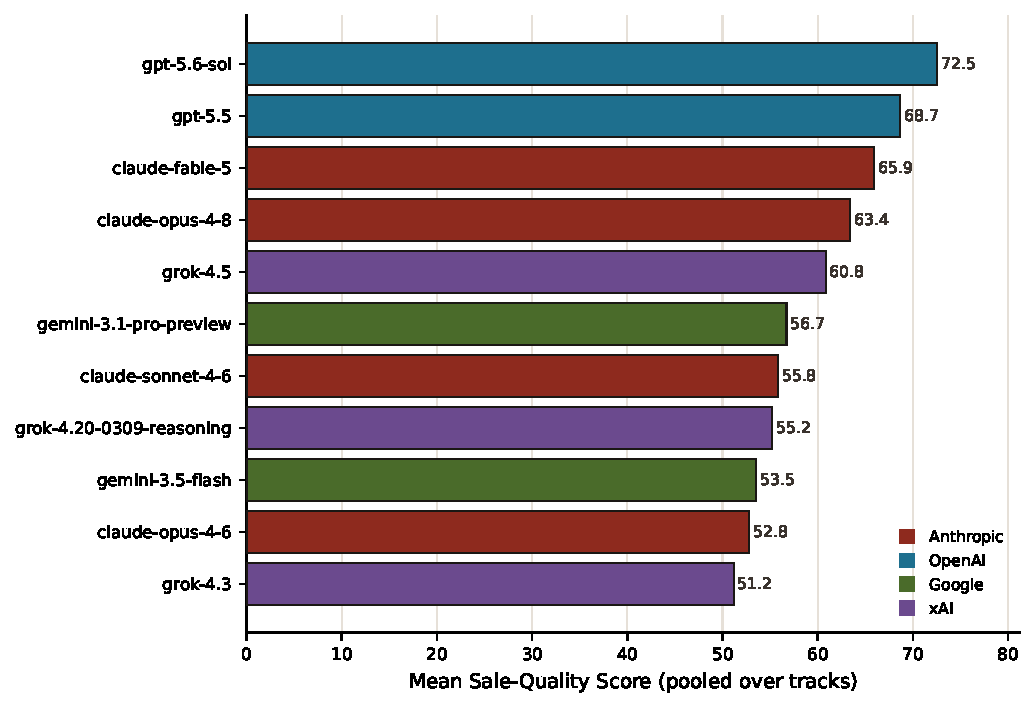
\includegraphics[width=0.82\linewidth]{figures/leaderboard_sqs.pdf}
  \caption{Mean Sale-Quality Score per model, pooled over both tracks and all
  tiers, colored by lab. The two OpenAI endpoints lead; the remaining field
  compresses into a $50$--$65$ band separated more by price discipline than by
  closing power.}
  \label{fig:leaderboard}
\end{figure}

\subsection{Methodology lift (OOB vs.\ pack)}
The headline paired comparison is the OOB$\to$pack lift with the model held fixed.
Pooled, the methodology pack changes clean-win rate by \resPackLiftOverall{}~pp.
Table~\ref{tab:lift} breaks the lift down by difficulty tier: \resLiftEasy{}~pp on
easy, \resLiftMid{}~pp on mid, and \resLiftHard{}~pp on hard. The SQS lift is
significant and largest on the easy tier ($+3.23$, $95\%$ CI $[+1.70,+4.77]$),
straddles zero on mid ($-1.10$) and hard ($+0.65$), and is positive but small when
pooled ($+1.21$, $95\%$ CI $[+0.29,+2.14]$). The methodology pack thus helps most
where the deal is \emph{winnable} and does not rescue structurally hard deals---the
opposite of the ``discipline matters most under pressure'' story, and a more honest
one: a prompt-injected playbook raises the floor on execution but cannot manufacture
access or budget that the scenario withholds. Mechanically, the pack's effect is
visible as a rise in economic-buyer engagement (EB-attended rate $30.0\%\to32.8\%$
pooled) and a marginal MAP-completion gain ($43.6\%\to44.5\%$); models that convert
the pack into \emph{behavior} (higher EB and MAP rates) gain, while those that
convert it only into \emph{vocabulary} do not.

% AUTO-GENERATED by analysis/gen-macros.py — do not hand-edit.
\begin{table}[t]
  \centering
  \caption{Methodology lift: paired OOB$\to$pack change in clean-win rate and mean
  SQS, by difficulty tier, with the model held fixed and seeds shared. Positive
  values indicate the methodology pack improved outcomes. The 95\% CI is a
  seed-matched paired bootstrap (5{,}000 resamples) on $\Delta$SQS; intervals that
  exclude zero are boldface. Lift is real but modest and concentrated in the easy
  tier: the pack helps most where the deal is winnable, and does not rescue
  structurally hard deals.}
  \label{tab:lift}
  \begin{tabular}{lcccc}
    \toprule
    Tier & Pairs & $\Delta$Clean-win\% & $\Delta$SQS & 95\% CI on $\Delta$SQS \\
    \midrule
    Easy (d1) &   780 & \resLiftEasy{}          & $+$3.18 & \textbf{[$+$1.82, $+$4.54]} \\
    Mid (d2)  &   585 & \resLiftMid{}           & $-$1.44 & \textbf{[$-$2.81, $-$0.09]} \\
    Hard (d3) &   390 & \resLiftHard{}          & $+$0.01 & [$-$1.60, $+$1.67] \\
    \midrule
    Pooled    &  1755 & \resPackLiftOverall{}   & $+$0.93 & \textbf{[$+$0.07, $+$1.81]} \\
    \bottomrule
  \end{tabular}
\end{table}


\subsection{Behavioral decomposition}
Beyond outcomes, we report the process metrics that SQS is built from: EB-meeting
attainment, MAP completion, and price integrity. Figure~\ref{fig:behavior} shows the
per-model behavioral fingerprint, and it tracks the leaderboard almost exactly. The
single strongest correlate of rank is economic-buyer engagement: \resBestModel{}
attains an EB meeting with conditional commitment on $71.9\%$ of pack runs and
confirms $64.4\%$ of MAP dates, whereas the bottom-ranked grok-4.3 reaches the EB on
only $5.2\%$ of runs and confirms $22.0\%$ of dates. The models that win are the
models that earn access and drive a plan; closing power is downstream of process
discipline, not a substitute for it.

\begin{figure}[t]
  \centering
  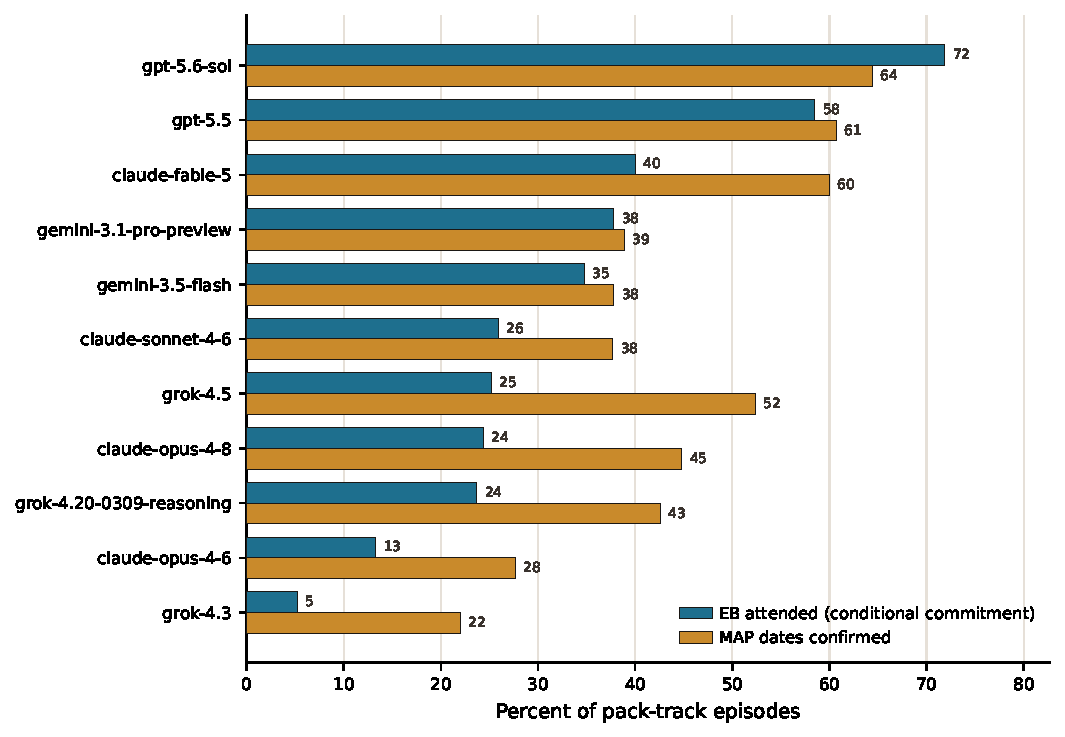
\includegraphics[width=0.9\linewidth]{figures/behavioral_fingerprint.pdf}
  \caption{Per-model behavioral fingerprint on the pack track: economic-buyer
  attainment (meeting with a conditional commitment on record) and mutual-action-plan
  date confirmation, sorted by EB attainment. The ordering mirrors the SQS
  leaderboard---closing power is downstream of earning access and driving a plan.}
  \label{fig:behavior}
\end{figure}

\subsection{Price discipline}
Mean discount conceded is \resDiscountOOB{}\% under OOB and \resDiscountPack{}\%
under pack---the pack slightly \emph{raises} mean discount and mean price-integrity
score edges down ($0.706\to0.685$ pooled), because the pack pushes models to engage
more aggressively on price-pressured, discount-bait deals rather than walking away
early. Price behavior is highly model-dependent: the discount-disciplined
claude-opus-4-8, grok-4.5, and claude-fable-5 hold price-integrity above $0.80$,
while gemini-3.5-flash collapses to $0.44$, gifting discounts across the episodes
it fails to close (its clean wins, by construction, held price) as noted above.

\subsection{Judge reliability}
Direct human-expert agreement ($\kappa$, $\alpha$) is a pre-registered, forthcoming
study (Section~\ref{sec:validation}). The reliability evidence in hand today is the
inter-panel calibration of Section~\ref{sec:panel-calibration}: on \resPanelCalibN{}
doubly graded trajectories the cost-reduced grading panel agrees with a frontier
reference panel at mean Pearson $r=\resPanelPearson{}$ (mean absolute difference
\resPanelMAD{} on a $0$--$1$ scale), and matches categorical labels on
\resPanelCatPosture{}--\resPanelCatEthic\% of cases. We release the paired
per-feature agreement table with the dataset and will publish the human-expert
$\kappa$/$\alpha$ addendum against the frozen sample manifest.

\subsection{Judge robustness: the hardened track}
\label{sec:hardened}
To bound the risk that the leaderboard is an artifact of a lenient or gameable
judge, we re-graded \resHardenedScope{} under a second, \emph{hardened} judge that
reconstructs the objective qualification dimensions---MEDDPICC coverage,
economic-buyer attainment, and MAP-date confirmation---deterministically from the
turn-indexed event log, and lets the LLM score only the irreducibly subjective
dimensions (trust, price integrity, champion quality). This removes the judge's
discretion over exactly the dimensions a model could most plausibly talk its way
into. The hardened judge re-scored \resHardenedCells{} of those cells (one cell
failed re-grade on a transient judge error and falls back to its default grade).
The re-grade predates the two open-weight arms and covers \resHardenedScope{}
rather than the full \gridCellsTotal{}-cell grid; we report its scope explicitly
rather than imply coverage it does not have. The result is a robustness check,
not a replacement: we report it as a parallel track and keep the default judge as
the primary ranking.

The rankings are stable. The mean per-model SQS change is
\resHardenedMeanDelta{}~points---the hardened judge is marginally \emph{stricter},
consistent with removing upward discretion---and the top of the board does not move
(\resHardenedRankChurn{} changes in the top two). The largest single drop is
\resHardenedMaxDropModel{} at \resHardenedMaxDrop{}~SQS: the model that most relied
on the judge's generosity on the subjective-adjacent process dimensions is exactly
the one the hardened judge marks down, while a handful of disciplined models
(claude-opus-4-6, grok-4.20-0309-reasoning) tick slightly \emph{up}. That the
ordering survives an adversarial re-grade is direct evidence that SQS tracks the
evidence in the transcript rather than the judge's latitude.

\subsection{Reward distribution: VEB as an RL environment}
\label{sec:distribution}
VEB is designed to double as a verifiable RL environment, so a first-order question
is whether its reward carries usable training signal. Reframing each rollout
(scenario $\times$ seed $\times$ track) as one ``problem'' with scalar reward
$r=\mathrm{SQS}/100\in[0,1]$,\footnote{This training reward $r=\mathrm{SQS}/100$ is
the evidence-graded sale-quality signal used throughout this section. It is distinct
from the environment's native per-rollout \texttt{reward} field---a milestone/DVI
composite with veto rules, documented per rollout in \texttt{reward\_breakdown}---which
the release also ships; the two have different grand means by construction.} we
examine the per-model reward distribution over all
\gridCellsTotal{} rollouts. The grand-mean reward is \resDistGrandReward{} with a
mean per-model spread of \resDistMeanStd{}, and---critically for RL---the reward is
neither saturated at $1$ (solved) nor collapsed at $0$ (impossible). The mean
normalized Shannon entropy of the per-model reward histogram is
\resDistMeanEntropy{} (10 bins), ranging from \resDistEntropyLo{} for the
low-variance grok-4.3 to \resDistEntropyHi{} for the high-variance gemini-3.5-flash.
A mid-to-high entropy band is the signature of an environment that discriminates:
even the leader (gpt-5.6-sol, mean reward \resDistLeaderReward{}) clears the
$\mathrm{SQS}\ge\resPassBar{}$ clean-pass bar on only \resDistLeaderPass{}\% of
rollouts, leaving substantial headroom, while weaker models produce a broad, non-
degenerate reward spread rather than an all-fail spike. This is exactly the
distributional shape preference-based post-training consumes: dense enough to
separate policies, hard enough to leave room to improve. We release the per-rollout
reward vectors so that binning, binarization at any bar, and entropy can be
recomputed downstream; the \texttt{/benchmark} companion renders these
distributions interactively under both judge tracks.
